\begin{frame}{caches}
    \begin{itemize}
    \item caches --- fast memory that holds\\
        \myemph{recently accessed values from main memory} and \\
        \myemph{values near recently accessed values from main memory}
    \item idea: program thinks it accesses main memory\ldots \\
        but most accesses take `shortcut' to cache
    \end{itemize} 
\end{frame}

\begin{frame}[fragile,label=observeCaches]{observing caches}
\lstset{
    language=C++,style=smaller
}
\begin{lstlisting}
unsigned run(int count) {
    unsigned index = 0;
    for (unsigned j = 0; j < count; ++j) {
        index = array[index];
    }
    return index;
}

// setup to access array with no easily observed pattern
    // NB: 103 will be relatively prime, so this accesses
    //     every element of the array
void setup(int size) {
    for (unsigned i = 0; i < size; ++i) {
        array[i] = ((i + 1) * 103) % size;

    }
}
\end{lstlisting}
\end{frame}

\begin{frame}{observing caches}
    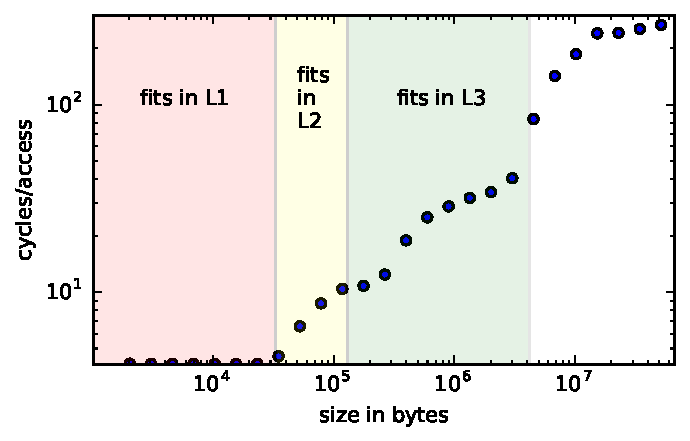
\includegraphics[width=\textwidth]{size-v-cycles}
\end{frame} 
